
%\chapter{Граница инерционного интервала и диссипативная область турбулентного каскада} \label{chapt3}
%
%\section{"Квазипланковский" спектр на поверхности жидкого водорода} \label{sect3_1}
%\section{Граница инерционного интервала на поверхности воды} \label{sect3_2}
%\section{Диссипативная область турбулентного каскада на поверхности воды} \label{sect3_3}

%abstract
%Экспериментально исследовано формирование вихревого течения в сосуде с жидкостью, совершаю-
%щем гармонические колебания в вертикальном направлении. Установлено, что в цилиндрическом сосуде вихревого течения не наблюдается до тех пор, пока амплитуда колебаний не превысит порогового значе- ния, при котором развивается параметрическая неустойчивость Фарадея и на поверхности появляются азимутальные моды. В квадратном сосуде и в цилиндрическом сосуде с нарушенной симметрией вих- ри наблюдаются при амплитудах ниже порога параметрической неустойчивости. Предполагается, что формирование вихревого течения обусловлено взаимодействием распространяющихся под углом друг к другу поверхностных волн.

%\epstopdfsetup{outdir=./images/article3/}

\chapter{Формирование вихревого течения капиллярными волнами на поверхности жидкости} \label{chapt3}

\section{Экспериментальная методика}\label{sect3_2}
Закрепленный на виброплатформе сосуд цилиндрической или квадратной формы заполняли дистиллированной водой. Глубина обоих сосудов 10мм, внутренний диаметр цилиндрического сосуда 65мм, сторона квадратного – 50мм. Сосуд совершал гармонические колебания по вертикали с амплитудой $S$ и частотой $omega_p$. В системе координат, связанной с сосудом, жидкость находится в переменном поле тяжести с ускорением, равным сумме ускорения свободного падения $g$ и переменного ускорения сосуда $g \beta cos(omega_p t)$, где $\beta = S \omega_p^2/g$ – безразмерная амплитуда переменного ускорения. Ускорение измеряли акселерометром, прикрепленным к стенке сосуда. В такой системе возможны два механизма рождения волн. Один из них связан с наличием мениска у поверхности жидкости, соприкасающейся с вертикальной стенкой сосуда. Мениск, периодически меняющий свою форму в переменном поле тяжести, служит источником поверхностной волны. Для эффективного возбуждения стоячей волны частота колебаний платформы $\omega_p$ должна быть близка к резонансной частоте колебаний поверхности жидкости в сосуде $\omega_n$. В цилиндрическом сосуде этим способом возбуждаются радиальные моды колебаний поверхности жидкости, которые описываются функцией Бесселя первого рода:

\begin{equation}
 %\label{eq:disperCap}
\eta(r, t) = \eta_0 cos(\omega_n t) J_0(k_n r)
\end{equation}

где n – номер резонанса, $k_n$ и $\omega_n$ – волновое число и частота моды, $\eta_0$ – амплитуда колебаний поверхности жидкости в центре сосуда. В квадратном сосуде плоские волны, распространяющиеся перпендикулярно от каждой стенки, образуют пару стоячих волн:

\begin{equation}
 %\label{eq:disperCap}
\eta(x, y, t) = \eta_x cos(\omega_n t) cos(k_n x) + \eta_y cos(\omega_n t) cos(k_n y) 
\end{equation}

Связь частоты и волнового числа определяется дисперсионным соотношением, в которое входят поверхностное натяжение $\sigma$ и плотность $\rho$ жидкости, а также глубина $h$ слоя [12]:

%\begin{equation}

% \label{eq:disper1}
%\omega^2 = (gk + \sigma/\rho k^3)tanh(kh),

%\end{equation}

Другой механизм возбуждения волн связан с параметрической неустойчивостью плоской поверхности жидкости в переменном поле тяжести. Для наблюдения параметрического резонанса частота вынужденных колебаний сосуда $\omega_p$ должна быть в два раза больше частоты резонансной моды $\omega_n$. Из-за наличия затухания поверхностных волн этот механизм в отличие от предыдущего является пороговым: усиления волны не происходит, пока амплитуда переменного ускорения не превысит критического значения $\beta_c$. Величина порога оказывается больше, если частота колебаний сосуда отличается от удвоенной резонансной частоты. При параметрическом возбуждении поверхностных волн в цилиндрическом сосуде, кроме радиальных мод (1), также могут возбуждаться и азимутальные моды:

\begin{equation}
 %\label{eq:disperCap}
\eta(r, \phi, t) = \eta_0 cos(\omega_n t) J_0(k_n r) cos(m \phi)
\end{equation}

Допустимые значения волновых чисел здесь определяются из условия отсутствия протекания жидкости через вертикальную стенку сосуда, $k_{n, m} = \mu_n^{(m)}/R$
где $n$, $m$ – целые числа, $R$ – радиус сосуда, $\mu_n^{(m)}$ – корни уравнения $J'_m(x) = 0$. Для визуализации течения на поверхности в воду добавляли порошок из полиамида PA12 со средним диаметром частиц 25–30 мкм либо стеклянные сферы диаметром 50мкм. Плотность стеклянных сфер была немного меньше плотности воды. Поверхность жидкости освещали фотовспышкой в стробоскопическом режиме и фотографировали с большой выдержкой. В результате получали изображения треков пробных частиц. Для нахождения горизонтальной составляющей скорости течения жидкости поверхность с пробными частицами фотографировали с частотой около 5.5 кадра/с при длительности фотовспышки 1мс. Поле скоростей определяли из парных изображений с помощью программы PIVlab [13]. Завихренность вычисляли как

\begin{equation}
 %\label{eq:disperCap}
\Omega(x, y) = \frac{\partial V_x}{\partial y} - \frac{\partial V_y}{\partial x}
\end{equation}
где $V_x$, $V_y$ – компоненты скорости в x- и y- направлениях. 

\section{Экспериментальные результаты и их обсуждение} \label{sect3_3} На рис. \ref{img:wave_rad} показана фотография поверхности воды, декорированной порошком из полиамида, в цилиндрическом сосуде. При колебаниях виброплатформы на частоте 25 Гц с амплитудой ниже пороговой для данной частоты на поверхности жидкости возбуждается радиальная мода $n = 6$ с длиной волны $\lambda \approx 10$ мм. В зависимости от плотности и смачиваемости пробные частицы дрейфуют либо к узлам, либо к пучностям стоячих волн [14]. На фотографии хорошо видны концентрические круги, сформированные частицами, которые собираются в узлах стоячей волны. Заметим, что на этом снимке вихревого движения не наблюдается. При постепенном увеличении амплитуды колебаний виброплатформы амплитуда колебаний поверхности жидкости плавно нарастает. При достижении некоторого значения амплитуды переменного ускорения $\beta$ наблюдается резкое усиление колебаний поверхности и возникает азимутальная мода (4) с числом $m$ порядка 10. Эту амплитуду переменного ускорения принимали за пороговое значение $\beta_c$. Появление азимутальной моды сопровождаетсяформированием вихревого движения на поверхности (рис. \ref{img:wave_az}). На фотографии отчетливо видна система из трех концентрических поясов вихрей. В каждом поясе содержится по 12 пар вихрей, вращающихся в противоположных направлениях. Наибольшие размеры имеют вихри внешнего пояса вблизи стенки сосуда. При дальнейшем увеличении амплитуды накачки возникают крупномасштабные течения, разрушающие концентрическое расположение вихрей.

\begin{figure}[ht] 
  \center
  \includegraphics [scale=1] {article3/pic_01.jpg}
  \caption{Фотография поверхности воды при колебаниях цилиндрического сосуда на частоте 25Гц с амплитудой, меньшей критической для возбуждения параметрического резонанса} 
  \label{img:wave_rad}  
\end{figure}

\begin{figure}[ht] 
  \center
  \includegraphics [scale=1] {article3/pic_02.jpg}
  \caption{Распределение вихрей на поверхности воды в цилиндрическом сосуде. Частота колебаний сосуда $\omega_p/2\pi = 45$ Гц, амплитуда переменного ускорения $\beta = 0.36$, пороговое ускорение $\beta_c = 0.26$. Видна азимутальная мода n = 4, m = 6, $\omega/2\pi = 22$ Гц} 
  \label{img:wave_az}  
\end{figure}




Переход от цилиндрического сосуда к сосуду квадратной формы радикально отражается на условиях формирования системы вихрей. На рис. \ref{img:vort_square} показаны распределения завихренности (5) на поверхности воды в квадратном сосуде при накачке на частоте 45.5 Гц до и после наступления параметрической неустойчивости. До порога $\beta/\beta_c \approx 0.9$ наблюдается симметричная система небольших вихрей (рис. \ref{img:vort_square}a), которые образуют квадратную решетку с периодом, равным длине поверхностных волн на частоте 45.5Гц ($\lambda \approx 6$ мм). Симметричная структура сохраняется и при незначительном превышении порогового значения ускорения, $\beta/\beta_c \approx 1.1$ (рис. \ref{img:vort_square}b). При дальнейшем повышении уровня накачки происходят слияние и укрупнение вихрей вследствие нелинейности.

\begin{figure}[ht]
  \begin{minipage}[ht]{0.49\linewidth}
    \center{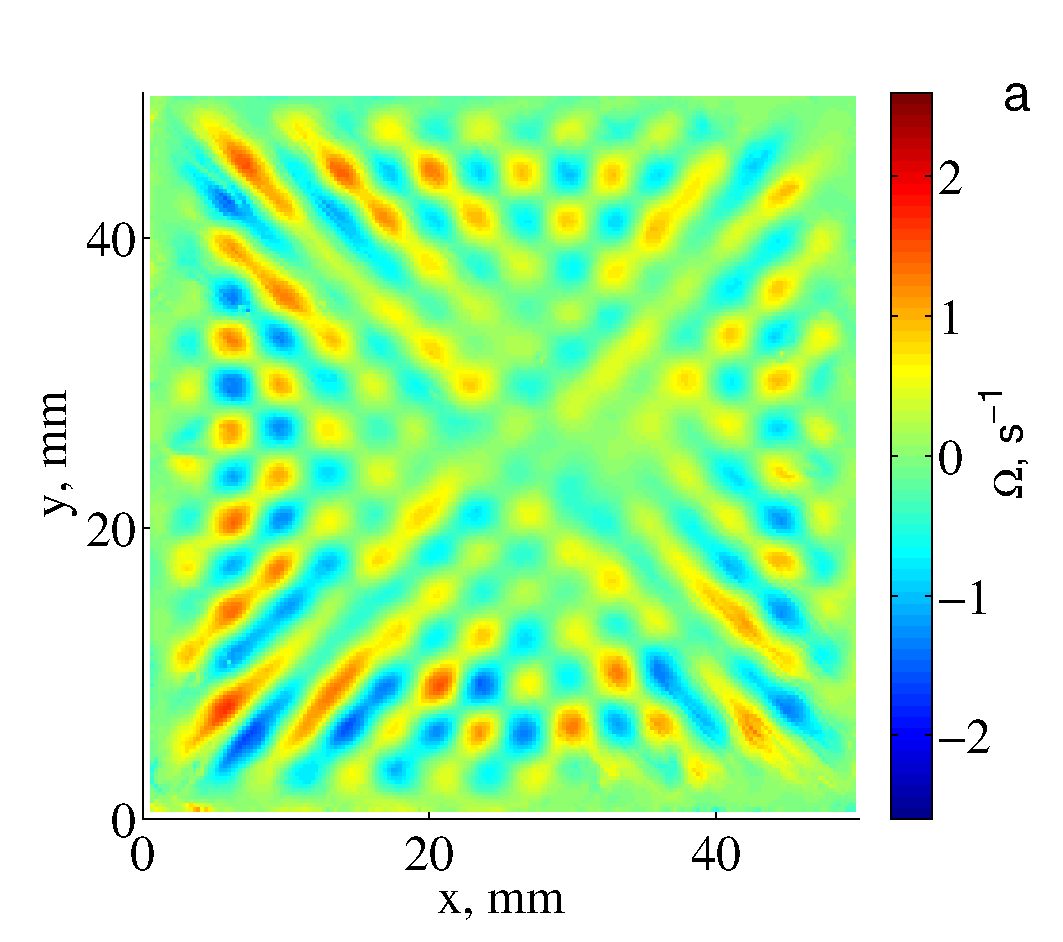
\includegraphics[width=1\linewidth]{article3/pic_03a.eps} \\ а)}
  \end{minipage}
  \hfill
  \begin{minipage}[ht]{0.49\linewidth}
    \center{\includegraphics[width=1\linewidth]{article3/pic_03b.eps} \\ б)}
  \end{minipage}
  \caption{Завихренность $\Omega$ на поверхности воды в квадратном сосуде при разных амплитудах колебаний на частоте 45.5 Гц: до порога возникновения параметрической неустойчивости (амплитуда переменного ускорения $\beta$ = 0.4, a) и после развития параметрической неустойчивости ($\beta$ = 0.48, b). Пороговое ускорение $\beta_c$ = 0.44}
  \label{img:vort_square}  
\end{figure}

На рис. \ref{img:fft_square} приведены фурье-образы вихревых структур, представленных на рис. \ref{img:vort_square}. При накачке с амплитудой, меньшей критического значения, на поверхности доминирует структура с обратным периодом $\approx 10$ см$^{-1}$ (рис. \ref{img:fft_square}a) в обоих направлениях, что соответствует волновому числу волны на частоте накачки. На рис. \ref{img:fft_square}b, помимо первоначальной структуры, видна структура с обратным периодом около 6 см$^{11}$, амплитуды Фурье которой в несколько раз превышают амплитуды Фурье первоначальной структуры. Возрастание периода решетки вихрей связано с появлением на поверхности воды стоячих волн с частотой $omega_p/2$, длина волны которых совпадает с периодом вихревой структуры, возникающей при переходе через порог неустойчивости Фарадея. 

\begin{figure}[ht]
  \begin{minipage}[ht]{0.49\linewidth}
    \center{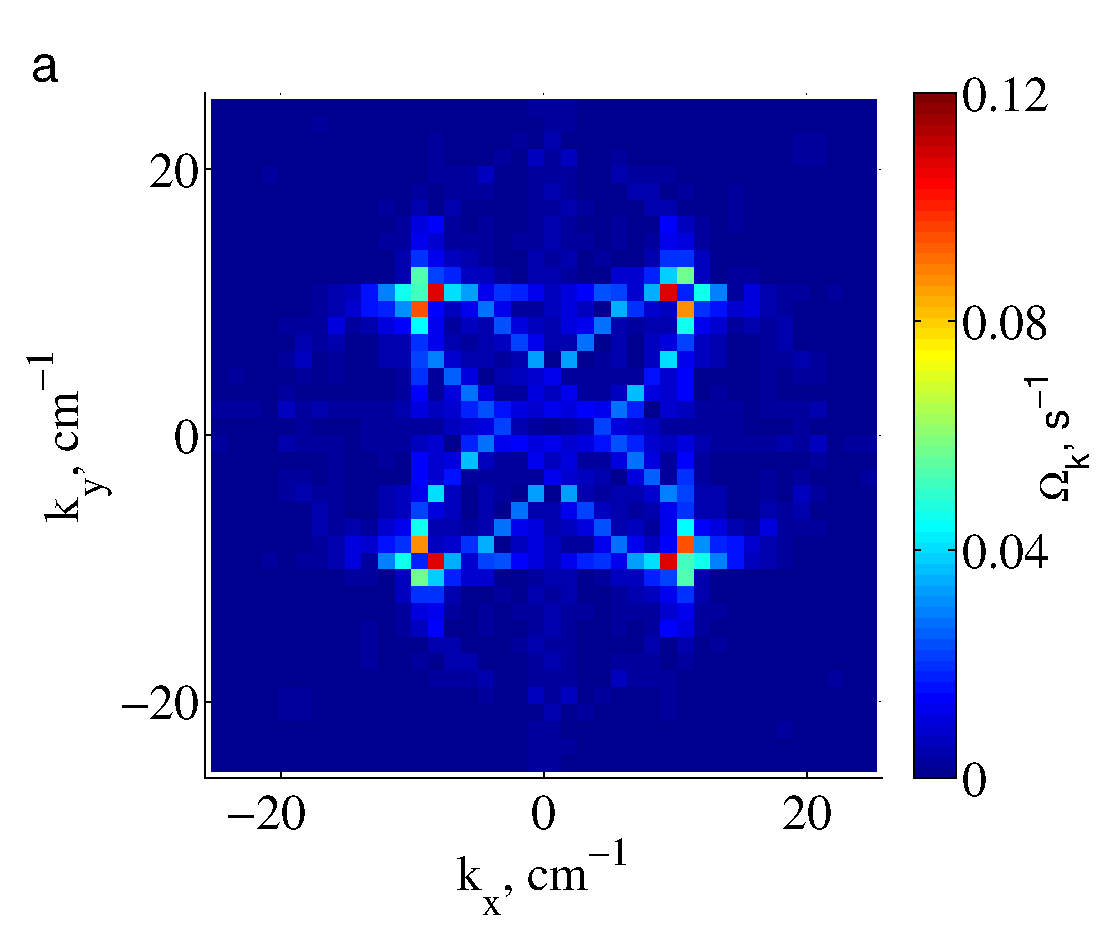
\includegraphics[width=1\linewidth]{article3/pic_04a.eps} \\ а)}
  \end{minipage}
  \hfill
  \begin{minipage}[ht]{0.49\linewidth}
    \center{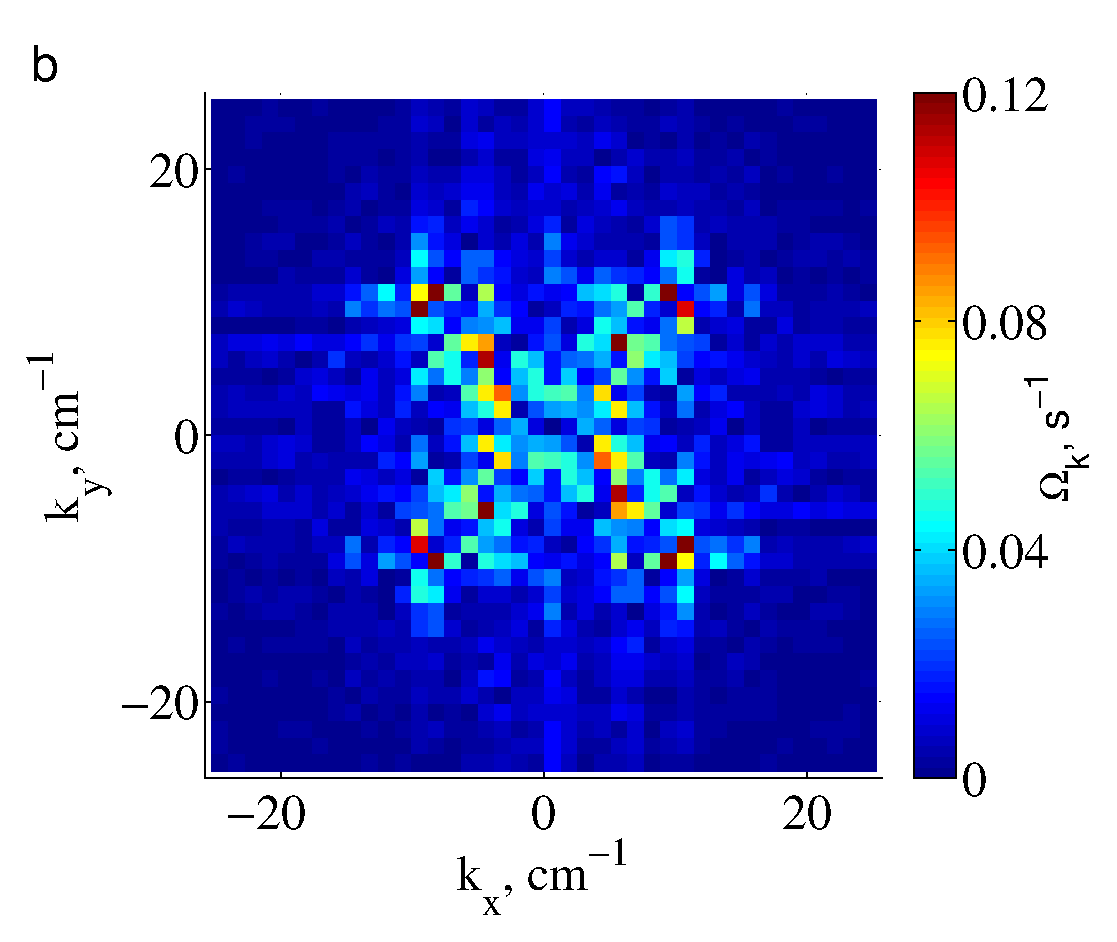
\includegraphics[width=1\linewidth]{article3/pic_04b.eps} \\ б)}
  \end{minipage}
  \caption{Завихренность $\Omega$ на поверхности воды в квадратном сосуде при разных амплитудах колебаний на частоте 45.5 Гц: до порога возникновения параметрической неустойчивости (амплитуда переменного ускорения $\beta$ = 0.4, a) и после развития параметрической неустойчивости ($\beta$ = 0.48, b). Пороговое ускорение $\beta_c$ = 0.44}
  \label{img:fft_square}  
\end{figure}

Зависимость интегральной завихренности $|\Omega|$ движения на поверхности воды от амплитуды переменного ускорения $\beta$ в квадратном сосуде показана на рис. 5. При изменении амплитуды переменного ускорения $\beta$ от 0.11 до 0.55 завихренность $|\Omega|$ возрастает почти на два порядка, причем ее быстрый рост наблюдается при ускорениях выше порога параметрической неустойчивости. При накачках ниже порогового значения изменение завихренности как функции амплитуды ускорения $\beta$ хорошо описывается степенной зависимостью $|\Omega| \sim \beta^{1.7}$. Поскольку при прочих равных условиях амплитуда возбуждаемых на поверхности стоячих волн $A$ прямо пропорциональна амплитуде переменного ускорения $\beta$, зависимость интегральной завихренности от амплитуды волн будет иметь тот же показатель. Оценка дает $|\Omega| \sim \beta^{2}$ [15]. Отличие, по-видимому, вызвано неоднородностью поля завихренности: вблизи края сосуда она больше, чем в центре (рис. \ref{img:vort_square}a).

Так как в квадратном сосуде вихревое движение наблюдается при амплитудах накачки значительно ниже порога параметрической неустойчивости, формирование вихревого движения здесь не может быть приписано особенностям параметрической неустойчивости Фарадея. Тот факт, что структуры вихревого и волнового движения коррелируют между собой, позволяет предположить, что волны непосредственно участвуют в формировании вихрей. Принципиальное отличие волн в квадратном сосуде, где вихри наблюдаются, начиная с самых малых амплитуд накачки, от волн в цилиндрическом сосуде, где вихри появляются только при достижении порога неустойчивости, связано с количеством одновременно возбуждаемых мод колебаний поверхностижидкости на фиксированной частоте. В квадратном сосуде ввиду симметричности всегда возбуждается пара мод (2). В цилиндрическом сосуде две разные моды, радиальная (1) и азимутальная (4), возбуждаются только после превышения порога параметрической неустой- чивости. Можно предположить, что изменение симметрии цилиндрического сосуда, которое приведет к возбуждению азимутальных мод при амплитудах накачки, меньших порогового значения, также сделает возможным формирование вихревого движения при этих же амплитудах.

\begin{figure}[ht]
  \begin{minipage}[ht]{0.49\linewidth}
    \center{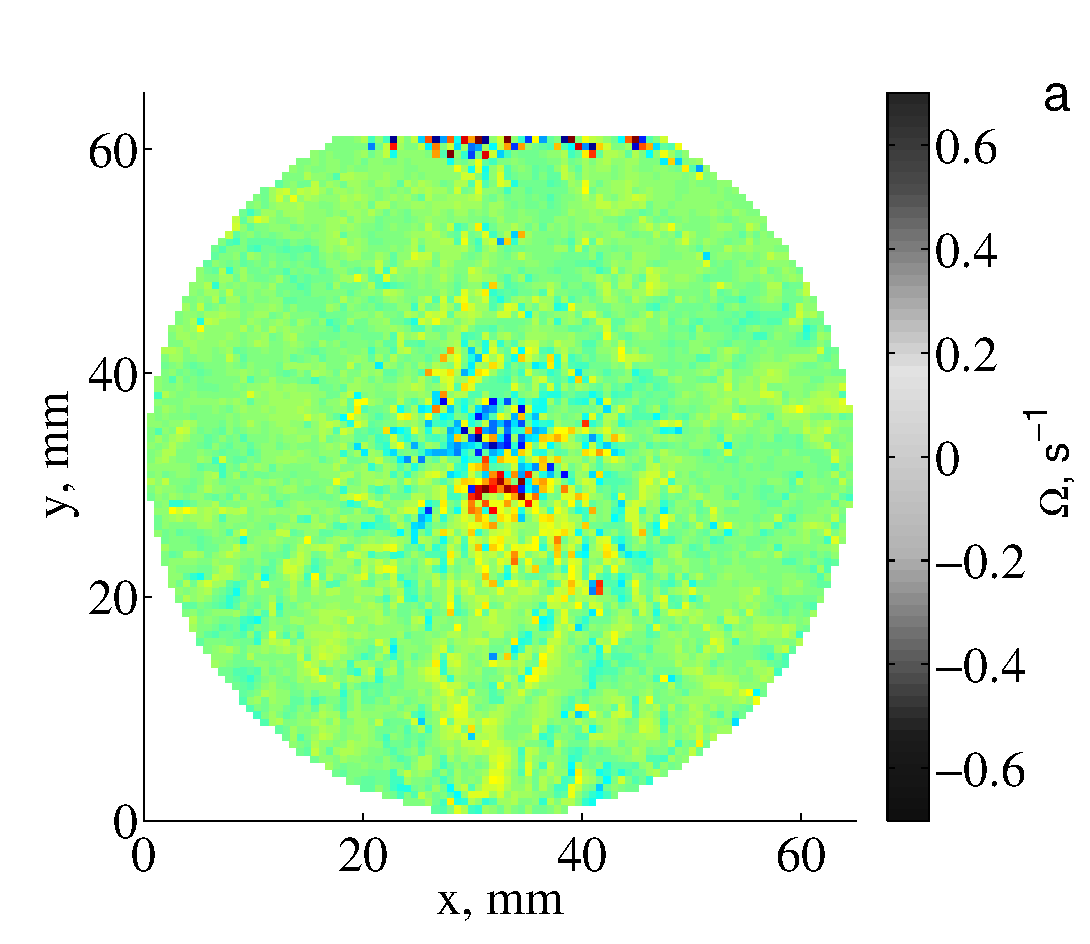
\includegraphics[width=1\linewidth]{article3/pic_06a.eps} \\ а)}
  \end{minipage}
  \hfill
  \begin{minipage}[ht]{0.49\linewidth}
    \center{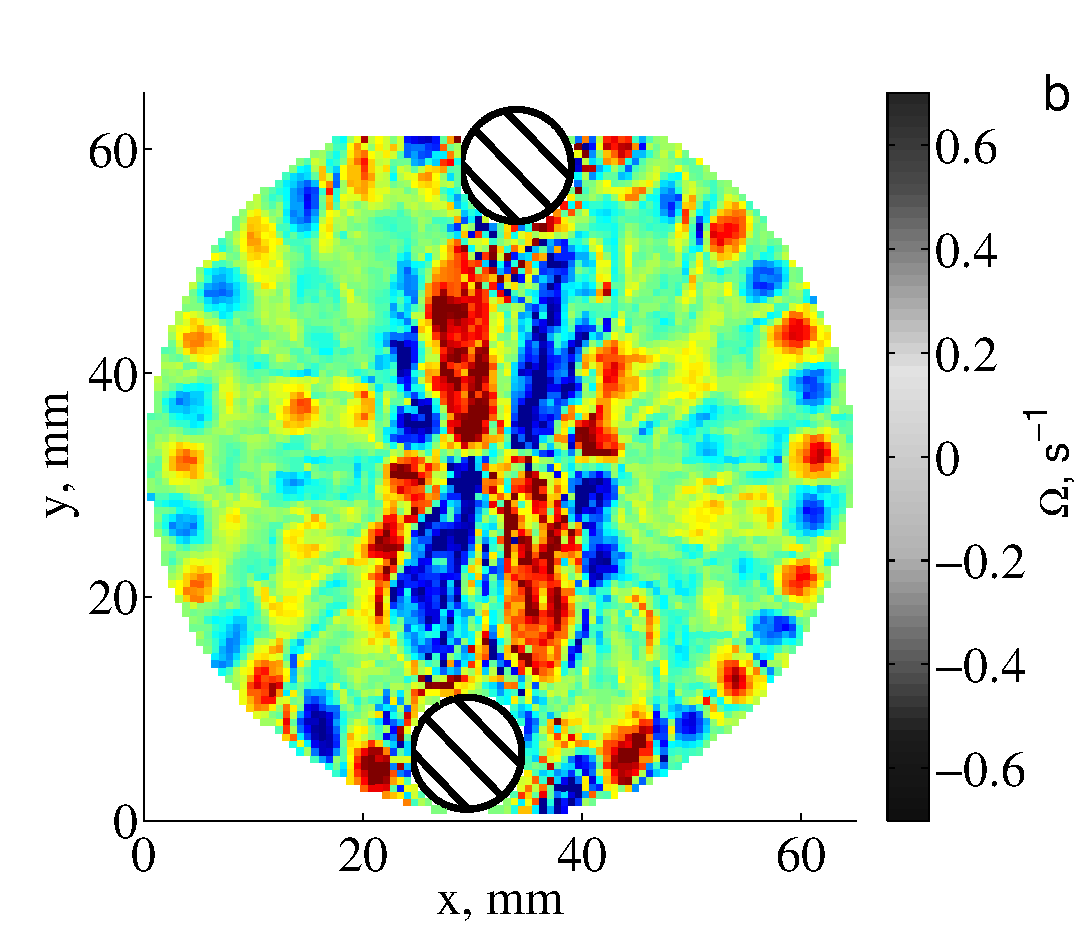
\includegraphics[width=1\linewidth]{article3/pic_06b.eps} \\ б)}
  \end{minipage}
  \caption{Поле завихренности $\Omega$ в цилиндрическом сосуде, в котором установлены два пластиковых столбика. На вставке – завихренность до установки столбиков. Цветовая шкала для завихренности общая.}
  \label{img:vort_st}  
\end{figure}

Для проверки данного предположения симметрия цилиндрического сосуда была нарушена установкой двух пластиковых столбиков диаметром 6.5мм, размещаемых диаметрально противоположно вблизи стенки сосуда. На рис. \ref{img:vort_st} показано поле завихренности до и после установки столбиков. В сосуде без вставок на поверхности жидкости возбуждается только радиальная волна и вихревого движения не наблюдается. После установки столбиков на поверхности хорошо возбуждаются азимутальные моды и появляется серия вихрей вдоль стенки сосуда аналогично системе вихрей на рис. \ref{img:wave_az}. Поскольку обе моды возбуждаются на одной частоте, их волновые векторы должны быть близки по модулю (в пределах резонансной ширины мод) и иметь разные направления. В квадратном сосуде независимо от частоты накачки угол между волно- выми векторами возбужденных волн составляет $90^\circ$. В цилиндрическом сосуде радиальную моду (1) на большом удалении от центра сосуда можно рассматривать как плоскую волну, волновой вектор которой направлен перпендикулярно стенке сосуда. Резонансную моду с малым радиальным числом $n$ и большим азимутальным числом $m$ по аналогии с модами шепчущей галереи для акустических волн можно рас- сматривать как распространяющуюся вдоль границы сосуда волну. Поэтому мы полагаем, что за формирование вихревого движения здесь отвечает взаимодействие двух поверхностных волн, волновые векторы которых направлены под углом друг к другу.
\section{Выводы} \label{sect3_3}
В настоящей работе экспериментально показано, что стоячие волны на поверхности жидкости в сосуде, который совершает гармонические колебания в вертикальном направлении с амплитудой переменного ускорения ниже порога параметрической неустойчивости, могут генерировать вихревое течение. В квадратном сосуде структура вихревого движения имеет вид квадратной решетки с периодом, равным длине стоячих волн. В цилиндрическом сосуде вихревое движение наблюдается только при возникновении азимутальных мод, которые возможны при амплитудах накачки выше порога рога параметрической неустойчивости. Искусственное понижение симметрии цилиндрического сосуда, которое разрешает генерацию азимутальных мод при малых амплитудах накачки, позволяет формировать вихревое движение при накачке значительно ниже порога параметрической неустойчивости Фарадея. Исходя из этих наблюдений и принимая во внимание степенную зависимость завихренности от амплитуды волн, можно утверждать, что в сосудах разной сим- метрии вихревое движение возникает тогда, когда на поверхностижидкости распространяется пара волн с неколлинеарными волновыми векторами.

\section{Нелинейное возбуждение завихренности поверхностными волнами} \label{sect3_3}
%Абстракт. Мы показываем, что волны, возбужденные на поверхности жидкости создают локальное вращение поврехности благодаря гидродинамической нелинейности. Мы исследовали теоретически этот эффект и получили точную формулу вертикальной завихренности с точки зрения отклонения высоты поверхности. Наши теоретические предсказания подтверждены измерениями поверхностного движения в ячейки с водой, где поверхностные волны возбуждались вертикальной гармонической тряской ячейки. Экспериментальные данные находятся в хорошем соответсвии с предсказаниями теории. Также мы обсуждаем физические следствия этого эффекта.

\section{Введение} \label{sect3_4}
Волны возбужденные на поверхности жидкости хорошо описываются с точки зрения потенциального движения жидкости. Это приближение обосновано слабостью волнового затухания. В этом случае ожидается, что завихренность жидкости будет ненулевой в узком слое около поверхности жидкости, где вязкость "уместна -relevant". В линейном приближении  завихренность направлена вдоль невозмущенной поверхности жидкости; следовательно её вертикальная компонента будет нулем, и все же наблюдается вихревое движение на поверхности жидкости возбуждаемое поверхностными волнами. Более сильные волны возбужденные с помощью неустойчивости Фарадея создают интенсивные вихревые поверхностные течения.

Однако, механизм возбуждения вихревых течений поверхностными волнами оставлся до сих пор неясным. Мы показали, что этот механизм связан с нелинейностью поверхностных волн. Можно грубо сказать, что наклон поверхности производит наклон вихря в вязком подслое. Впервые разработана теория объясняющая генерацию поверхносного вихревого движения повехностными волнами. Для простейшего случая двух плоских поверхностных волн теория была проверена экспериментально.

Мы показываем, что поверхностные волны близких частот могут генерировать повехностные вихревые течения слабо меняющиеся со времением и меняющиемся в пространстве на масштабе длины волны. Оказывается, что скорость связанная с течениями может быть описана как $v^2k/\omega$, где $v$ - поверхностная скорость в возбужденных волнах, $k$ - их волновой вектор и $\omega$ - частота этих волн. Удивительно, но выражение для скорости не зависит от вязкости, хотя оно выводится из вязкого механизма. Это свойство можно сравнить с гидродинамической турбулентностью. Её характеристики в инерционном интервале не зависят от вязкости, хотя вязкое затухание обеспечивает статистическую стационарность каскада.

Давайте рассмотрим нашу теоретическую схему. Объемное движение несжимаемой жидкости описывается уравнением Навье-Стокса:

\begin{equation}
 %\label{eq:disperCap}
\partial_t \mathbf{v} + (\mathbf{v \nabla})\mathbf{v} = - \mathbf{\nabla}P/\rho + \nu \mathbf{\nabla}^2\mathbf{v},
\end{equation}

где $\rho$ и $\nu$ плотность жидкости и коэффициент кинематической вязкости соответственно, $\mathbf{v}$ - скорость жидкости и $P$ - давление. Уравнение (1) должно быть дополнено условим несжимаемости $div \mathbf{v} = 0$. Уравнение для завихренности, $\varpi = curl \mathbf{v}$:

\begin{equation}
 %\label{eq:disperCap}
\partial_t \mathbf{\varpi} = -(\mathbf{v \nabla})\mathbf{\varpi} + (\mathbf{\varpi \nabla})\mathbf{v} + \nu \mathbf{\nabla}^2\mathbf{\varpi},
\end{equation}

Уравнение Навье-Стокса должно быть дополнено граничными условиями на поверхности жидности. Во-первых это "условие кинематической границы"

\begin{equation}
 %\label{eq:disperCap}
\partial_t h = v_z - v_x \partial_x h - v_y \partial_y h,
\end{equation}
подразумевая, что поверхность жидкости движется со скоростью жидкости $\mathbf{v}$. Здесь и далее мы предпологаем, что ось Z направлена вертикально против направления ускорения свободного падения $g$ и невозмущенная поверхность воды соответствует плоскости $z = 0$. Отклонение полверхности от положения равновесия описывается с поломощью высоты $h(x, y, t)$

Также есть динамическое граничное условие, которое может быть получено из требования "нулевого потока импульса " через поверхность жидкости Это приводит к условиям:

\begin{equation}
 %\label{eq:disperCap}
P - 2 \rho \nu n_i n_k \partial_i v_k = \rho g h + \sigma(\mathbf{\nabla n}),
\end{equation}

\begin{equation}
 %\label{eq:disperCap}
(\delta_{ij} - n_i n_j) n_k(\partial_j v_k + \partial_kv_j) = 0,
\end{equation}
которые должны удовлетворяться в точке $z = h$. Здесь - $\sigma$ коэффициент поверхностного натяжения и $\mathbf{n}(t, x, y) = (-\partial_x h, - \partial_y h, 1)/\sqrt{1+(\nabla h)^2}$ - единичный нормальный к поверхности вектор. Граничное условие для завихренности $\varpi_i = \epsilon_{ijk}\partial_jv_k$ следует из уравнения (5)

\begin{equation}
 %\label{eq:disperCap}
n_m n_k \partial_k \varpi_m = (\partial_i v_k + \partial_k v_i) \epsilon_{imn} n_m K_{kn} = 0,
\end{equation}

где $\epsilon_{ijk}$ единичный антисиммитричный терзор и мы ввели "тензор кривизны" $K_{ik} = K_{ki} = (\delta_{ij} - n_i n_j) \delta_j n_k$.

Далее мы рассмотрим случай где волны возбуждены на поверхности жидкости. Случай глубикой воды подразумевается. Мы предполагаем, что крутизна волны мала, т.е. $|\nabla h| \ll 1$. В линейном приближении мы имеем дело с гравитационно-капиллярными волнами, характерезующимися законом диспресии $\omega^2 = g k + (\sigma/\rho)k^3$, где $k$ - волновой вектор волны и $\omega$ - её частота. Мы также предполагаем, что волны слабо затухают, т.е. $\gamma = \sqrt{\nu k^2/\omega} \ll 1$.

В линейном приближении, все количественные характеристики поверхностных волн могут быть описаны через высоты поверхности $h$. "Явные" выражения для скорости и завихренности в первом порядке по малому параметру $\gamma$:

\begin{equation}
 %\label{eq:disperCap}
 v_\alpha = \nu[(\hat{\kappa}^2 + \hat{k}^2)/\hat{k}]exp(\hat{k}z)\partial_\alpha h - 2\nu \hat{\kappa} exp(\hat{\kappa}z) \partial_\alpha h,
\end{equation}

\begin{equation}
 %\label{eq:disperCap}
 v_z = \nu(\hat{\kappa}^2 + \hat{k}^2)exp(\hat{k}z)h - 2\nu \hat{\kappa}^2 exp(\hat{\kappa}z) h,
\end{equation}

\begin{equation}
 %\label{eq:disperCap}
\varpi_\alpha = 2 \epsilon_{\alpha \beta} exp(\hat{\kappa}z) \partial_\beta \partial_t h,
\end{equation}
см, например [1]. Здесь и далее греческие индексы бегут по $x$ , $y$ , $\epsilon_{\alpha\beta}$ - это единчный антисиммитричный тензор и вводим нелокальные операторы $\hat{k}^ = (-\partial_x^2 - \partial_y^2)^{1/2}$, $\hat{\kappa} = (\partial_t/\nu + \hat{k}^2)^{1/2}$. Первые члены в выражениях (7) и (8) относится к потенциальной части скорости, в то время как последние слогаемые соответствуют поправкам, возникающим из-за вязкости. Заметим, что завихренности $\varpi_\alpha$ сосредоточена в относительно тонком слое около поверхности. Глубина слоя описывается, как $\gamma/k \ll 1/k$, где $1/k$ глубина проникновения потенциальной части скорости.

Вертикальная составляющая завихренности $\omega_z$ равна 0 в линейном приближении, она возникает только из-за нелинейного взаимодействия волн. Следовательно, для того, чтобы найти $\omega_z$ следует выйти за рамки приближения. Мы принимаем во внимание основной нелинейной вклад в $\omega_z$ в ур-ние (2), где второй порядок в волновой амплитуде будет:
\begin{equation}
 %\label{eq:disperCap}
(\partial_z^2 - \hat{\kappa}^2)\varpi_z = -\nu^{-1} \varpi_\alpha \partial_\alpha	v_z.
\end{equation}

Слогаемое в правой части можно рассматривать как способ для нахождения $\omega_z$. Он соответсвует вращению двумерного вектора $\omega_\alpha$ из-за поля скорости поверхностных волн. Мы сохраняем нелинейные члены одного и того же порядка в граничном условии (6):

\begin{equation}
 %\label{eq:disperCap}
\partial_z \varpi_z = \partial_\alpha h \partial_z \varpi_\alpha - \epsilon_{\alpha \gamma}(\partial_\alpha v_\beta + \partial_\beta b_\alpha) \partial_\beta \partial_\gamma h.
\end{equation}

Заметим, что второе слагаемое в правой части уравнения (11) меньше, чем первое по параметру $\gamma$. Однако второе слагаемое стоит оставить, так как оно может дать значительный вклад в поверхностное значение $\varpi_z$, так как оно может создавать поправку имеющею большую глубину проникновения, см [7].

Решением уравнения (10) с граничными условиями (11) ( которые поставлены при $z = 0$) и $\varpi_z \to 0$ при $z \to -\infty$ будет:

\begin{equation}
 %\label{eq:disperCap}
\varpi_z(z) = 2 \epsilon_{\alpha \beta}(e^{\hat{k}z}\partial_\alpha h) (e^{\hat{k}z}\partial_\beta \partial_t h) + 2 \epsilon_{\alpha \beta} \hat{\kappa}^{-1}e^{\hat{\kappa}z}(\partial_\alpha h \partial_\beta \partial_t \hat{k}h + \partial_\alpha \partial_\gamma h \partial_\beta \partial_\gamma \partial_t \hat{k}^{-1} h),
\end{equation}
где были использованы уравнения (7)-(9). Поверхностное значение завихренности $\varpi$ были получены подстановкой $z=0$ в выражение (12). Первый член в выражении (12) отвечает за наклон завихренности (9) возникающий из-за наклона поверхности. Первый член в последних круглых скобках возникает в результате распростронения повернутой завихренности в объеме. Последний член в выражение (12) относится к ненулевой кривизне поверхности, который увеличивает дополнительную вязкость тангенциальной поверхностной силы.

Заметим, что, согласно уравнению (12) одиночная плоская поверхностная волна не создает завихренности $\varpi$, ненулевая $\varpi$ возникает, если возбуждены как минимум две плоские волны распространиющиеся в разных направлениях. Характерная частота $\omega_\nu$ завихренности $\varpi$ может варьироваться от нуля до значения порядка частоты поверхностной волны $\omega$ в рамках рассмотрения нелинейности второго порядка. Если $\omega_\nu \gg \nu k^2$, то первый член в правой правой части уравнения (12) основной. В противном случае оба члена одного порядка.

В дальнейшем мы анализируем случай, когда возбужденные поверхностные волны характерезуются узким спектром около $\omega$ с шириной $\Delta omega \ll \omega$. Тогда медленно меняющийся вклад в вертикальную завихренность $\varpi_z$ основной и таким образом $\omega_\nu \sim \Delta \omega$. Действительно из уравнения (12) следует, что относительная амплитуда вклада удвоенной частоты меньше, чем $\Delta \omega / \omega$ ; см. ссылку [7]. Дальше мы предполагаем, что $\omega_nu \ll \nu k^2$. В этом случае можно подставить $\kappa$ в $k$ во второй строчке уравнения (12). Таким образом, первый член в правой части уравнения (12) локализован на масштабе $\gamma/k$ около поверхности, в то время как второй член проникает глубже на расстояние $1/k$. Оба члена имеют сравнимые амплитуды на поврехности.

Сформулируем условия применимости нашей теории... Мы должны оценить нелинейные члены из уравнения (2), где второй порядок членов по скорости, $v^{(2)}$, должны быть приняты во внимание. Из уравнения (12) следует, что $v^{(2)} \sim \omega k h^2$. Следовательно... Таким образом в случае... Условия могут быть переписаны как $kh \ll 1$.

Перейдем к экспериментальной части. Для проверки теоретических предсказаний...

\begin{figure}[ht] 
  \center
  \includegraphics [scale=1] {article4/pic_01.jpg}
  \caption{} 
  \label{img:setup}  
\end{figure}

Стационарный паттерн стоячих капиллярных волн формируется в течении 1-2 с после включения возбуждения. Одновременно с рябью возникает квадратная решетка вихрей на поверхности. Вся картина остается стабильной по крайней мере в течение нескольких минут. Результаты эксперимента представлены на рис. \ref{img:vort_chess} и \ref{img:vort_roll} показана завихренность $\varpi_z$ усредненная по времени. Красный цвет соотвествует положительной завихренности, синий цвет - отрицательной завихренности, цветовая шкала определяющая значение звихренности так же представлена на рисунке.

\begin{figure}[ht] 
  \center
  \includegraphics [scale=.5] {article4/pic_02.eps}
  \caption{Завихренность в ячейке 50 x 49 мм$^2$ при возбуждении поверхностных волн с частотой 42.7 Гц. Наблюдается шахмотноподобный паттерн поля завихренности соответсвтующий теоретическому выражению (14). Период решетки в Х и У направлениях равно длинне волны.} 
  \label{img:vort_chess}  
\end{figure}

\begin{figure}[ht] 
  \center
  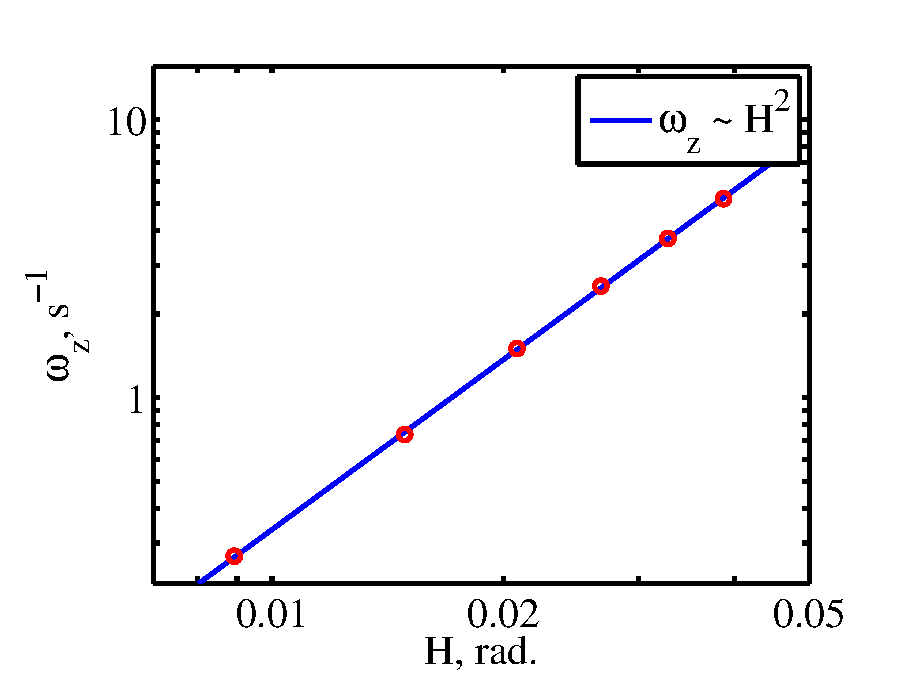
\includegraphics [scale=.5] {article4/pic_04.eps}
  \caption{Завихренность в ячейке 40 х 40 мм $^2$ при возбуждении поверхностных волн с частотой 54 Гц. Две стенки ячейки соответствующие левой и нижней части рисунка немного ниже, чем остальные станки. Уровень воды скорректирован, чтобы в основном возникало две бегущие волны от более низких стенок. Знакопеременные полосы положительной и отрицательной завихренности, направленные параллельно диагонали квадратной ячейки, согласуются с теоретическим выражением (16).} 
  \label{img:vort_roll}  
\end{figure}


Для объяснения рисунка сначала заметим, что силы действующие на волны относятся к мениску воды сформированному около стенки. Следовательно, эти силы локализованы около стен и можно использовать свободные гидродинамические уравнения для описания движения воды не очень близко к стенам. Мы имеем дело с почти линейными волнами заданной частоты, амплитуда волн определяется пристенными силами и граничными условиями. В ячейке возникают только волны распростаняющиеся перпендикулярно от стенок прямоугольной ячейки. Резонасные частоты соответсвуют волнам с длиной волны соответсвующей граничному условию: длина стенок ячейки равна целому числу длин волн с точностью до некоторой поправки, связанной с пристеночной областью. Линейный размер сосуда достаточно мал, чтобы расстояние в частотном пространстве между соседними резонансами было больше, чем ширина резонансов.  Волны распростроняющиеся в других направлениях не возбуждаются, так как мощность передаваемая от мениска волне в этом случае равна нулю.

На рисунке \ref{img:vort_chess} показана завихренность наблюдаемая в почти квадратной ячейке, где стоячие волны возбуждаются в $X$ и $Y$ направлениях. Пренебрегая затуханием волн, мы можем моделировать высоту жидкости как:

\begin{equation}
 %\label{eq:disperCap}
h = H_1 cos(\omega t) cos(kx) + H_2 cos(\omega t + \phi) cos(ky),
\end{equation}
где $k$ определяется законом дисперсии. Фазовый сдвиг $phi$ в уравнении (13) возникает из асимметрии ячейки, которая приводит к разным граничным условиям для стоячих волн в $X$ и $Y$ направлениях. Изменяя соотношение сторон ячейки можно менять разность фаз $phi$. Подставляя выражение (13) в уравнение (12) получаем:

\begin{equation}
 %\label{eq:disperCap}
\varpi_z(0) = -(2 + sqtr{2})sin \phi H_1 H_2 \omega k^2 sin(kx)sin(ky).
\end{equation}
Этот результат не зависит от времени.Сумма рациональных и иррациональных чисел соответствует сумме двух слагаемых в уравнении (12), которые имеют различную глубину проникновения. Это выражение (14) качественно соответсвует рисунку \ref{img:vort_chess}.

Мы также проводили эксперименты с квадратной ячейкой, где разница фаз $\phi \ll 1$  и распределение завихренности изменялось существенно. Для описания ситуации следует учитывать затухание волны вдоль направления распространения волны из-за вязкого затухания. Детали представлены в Дополнительной материала [7].

Амплитуда завихренности как функция волновой амплитуды показана на рисунке \ref{img:vort_ampl}. Высота отклонения поверхности вызванная волнами была измерена лазерным лучом отраженным от жидкой поверхности. Размер лазерной проекции на экран может быть пересчитан в амплитуду наклона поверхности $kH$, где $H$ амплитуда наибольшей волны. График на рисунке \ref{img:vort_ampl} показывает квадратичную зависимость завихренности от угловой амплитуды волны, что соответсвует нашим теоретическим предсказаниям.

\begin{figure}[ht] 
  \center
  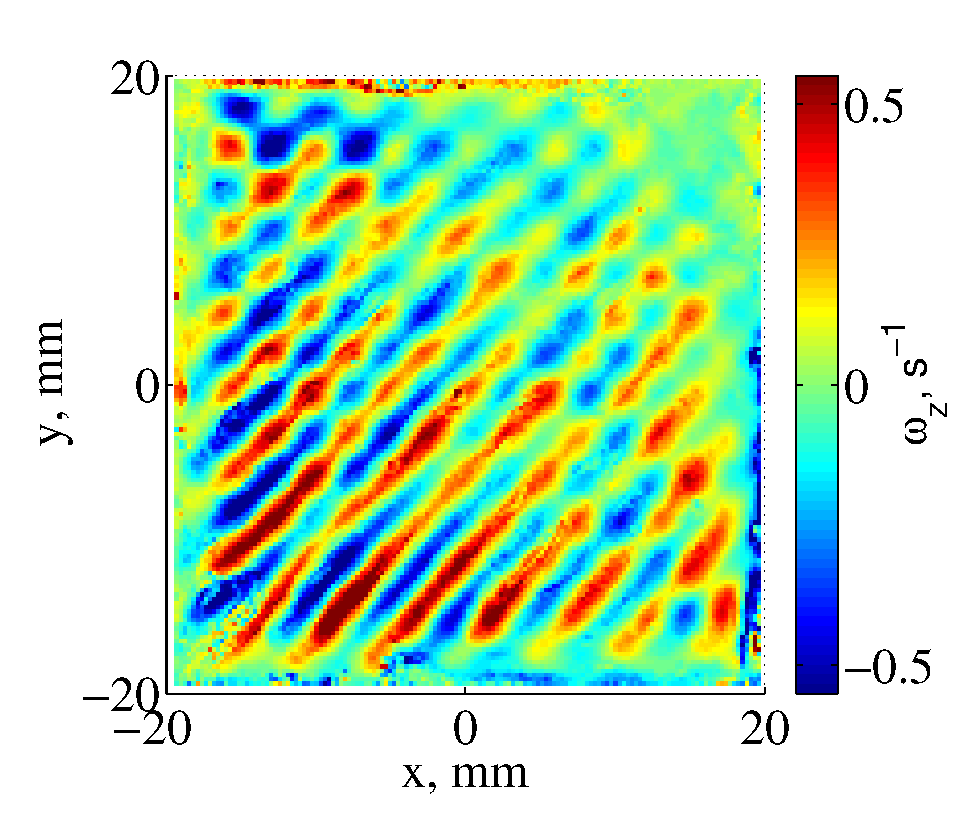
\includegraphics [scale=.5] {article4/pic_03.eps}
  \caption{Завихренность для различных амплитуд накачки в ячейке 50 x 49 мм$^2$, где возбуждаются поверхностные волны с частотой 42.7 Гц, строится в зависимости от амплитуды наклона $kH$. Линия соответствует зависимости $varpi \sim kH^2$ и доказывает, что завихренность генерируется нелинейностью второго порядка.} 
  \label{img:vort_ampl}  
\end{figure}

Рисунок \ref{img:vort_roll} показывает результат другого эксперимента. В этом эксперименте квадратная ячейка имела стенки с разной высотой: две смежные стенки немного ниже, чем две противоположные стенки. Для устранения мениска ячейка была наполнена водой точно по край высоких стенок. На низких стенках вода образует выпуклый мениск(см рис \ref{img:setup}с). Таким образом возбуждающие силы приложены исключительно на низких стенках. Пренебрегая эффектом отраженных волн, можно получить грубую модель распростроняющихся от низких стенок волн. Тогда отклонени поверхности будет задано как:

\begin{equation}
 %\label{eq:disperCap}
h = H_1 cos(\omega t - kx) + H_2 cos(\omega t - ky),
\end{equation}
Подставляя выражение (15) в уравнение (12) находим:

\begin{equation}
 %\label{eq:disperCap}
\varpi_z(0) = -(2 + sqtr{2})sin \phi H_1 H_2 \omega k^2 sin(kx-ky).
\end{equation}
Заметим, что результат так же не зависит от времени. Рисунок \ref{img:vort_roll} показывает, что пространсвенное затухание волн имеет значение. Учет затухания корректирует выражение (16), что приводит к разумному согласию между экспериментальными данными и теоретическими предсказаниями [7]. 

Заключение. Мы открыли новый механизм генерации поверхностной завихренности связанный с узким вязким слоем формируемой распростроняющимися поверхностными волнами. В частности этот механимз приводит к перемешиванию поверхности, которое может быть характерезовано как диффуззионным коэффициентом $D$ соответсующиего четвертому порядку волновой амплитуды, так из прямым действием волн на поверхности жидкости [9, 10]. Данная задача требует дальнейшего исследования. Несмотря на то, что эксперименты производились в капиллярной области, наши теоретические построения также применимы и в на гравитационной области. Для примера соответстующая теория может быть использована для анализа вихревого движения на поверхности океана.

Увеличивая амплитуду тряски ячейки можно достичь порога неустойчивости Фарадея. Значительно выше порога, поверхностные волны весьма интенсивны, что приводит к интенсивным вихревым движениям поверхности жидкости, для которых безразмерный параметр $\kappa h > \sim 1$. Тогда самовзимодействие вихревых движений становится значительным [11], что приводит, в частности, к образованию обратного каскада энергии [4]. Результаты наших теоретических и экспериментальных исследований позволяют лучше понять это явление и разработать количественную основу для него.

\clearpage